\begin{frame}{第十七讲、微分中值定理及其应用}
	\linespread{1.5}
	\begin{enumerate}
	  \item {\bf 内容与要求}{\b( \S 5.2 )}
	  \begin{itemize}
	    \item 熟练掌握Rolle定理和Lagrange中值定理
	    \item 理解Cauchy中值定理
	    \item 熟练掌握L'Hospital法则
	  \vspace{1em}
	  \end{itemize}
	  \item {\bf 课后练习:}
	  \begin{itemize}
	    \item 书面作业:{\b 习题5.2:3,7,9,11,14,17}
 	    \item 思考题:{\b 习题5.2:2,5,8,10,12,13,15,16,18}
	  \end{itemize}
	\end{enumerate}
\end{frame}

\section{Rolle定理}

\begin{frame}{Rolle定理}
	\linespread{1.2}\pause 
	\begin{block}{{\bf 定理5.2.1}\hfill P234}
		若函数$f(x)$满足:\pause 
		\begin{enumerate}
		  \item 在区间$[a,b]$上连续\pause 
		  \item 在区间$(a,b)$内可导\pause 
		  \item $f(a)=f(b)$\pause 
		\end{enumerate}
		则:存在$\xi\in(a,b)$,使得$f\,'(\xi)=0$。
	\end{block}\pause 
	{\bf 注:}\alert{以上三个定理条件缺一不可!}
\end{frame}

\begin{frame}
	\linespread{1.2}
	\begin{exampleblock}{{\bf 例1}\hfill}
		证明:对函数$f(x)=(x-1)(x-2)(x-3)$,至少存在一点
		$\xi\in(1,3)$,使得$f\,''(\xi)=0$。
	\end{exampleblock}
	\bigskip
	\pause
	\begin{block}{{\bf 推论}(Rolle定理的高阶推广)\hfill}
		设$f(x)$在$[x_0,x_n]$上有$n-1$阶连续导数,在$(x_0,x_n)$内
		$n$阶可导,且
		$$f(x_0)=f(x_1)=\ldots=f(x_n),\quad(x_0<x_1<\ldots<x_n),$$
		则存在$\xi\in(x_0,x_n)$,使得$f^{(n)}(\xi)=0$。
	\end{block}
\end{frame}

\section{Lagrange中值定理}

\begin{frame}{Lagrange中值定理}
	\linespread{1.2}\pause 
	\begin{block}{{\bf 定理5.2.2}\hfill P235}
		若函数$f(x)$满足:\pause 
		\begin{enumerate}
		  \item 在区间$[a,b]$上连续\pause 
		  \item 在区间$(a,b)$内可导\pause 
		\end{enumerate}
		则:存在$\xi\in(a,b)$,使得\pause 
		$$f\,'(\xi)=\df{f(b)-f(a)}{b-a}.$$
	\end{block}
\end{frame}

\begin{frame}%{Lagrange中值定理的应用}
	\linespread{1.2}\pause 
	\begin{block}{{\bf 推论}\hfill P237-例1}
		导数恒为零的函数取值恒为常数。
	\end{block}
	\bigskip
	\pause 
	\begin{exampleblock}{{\bf 例2}\hfill}
		证明:$\df{\ln x-\ln x_1}{x-x_1}<\df 1{x_1},\quad (0<x_1<x)$
% 		\begin{enumerate}
% 		  \item $\df{\ln x-\ln x_1}{x-x_1}<\df 1{x_1},\quad (0<x_1<x)$
% 		  \item $\limx{\infty}\df{\ln x}{x}=0$
% 		\end{enumerate}
	\end{exampleblock}
	\pause 
	\begin{exampleblock}{{\bf 例3}\hfill P237-例2}
		证明不等式:
		$$\df{x}{1+x}<\ln(1+x),\;x>0$$
	\end{exampleblock}
\end{frame}

\begin{frame}
	\linespread{1.5}
	\begin{exampleblock}{{\bf 例4}\hfill P237-例3}
		证明方程$x^5+x-1=0$只有唯一实根。
	\end{exampleblock}
	\bigskip
	\pause 
	\begin{exampleblock}{{\bf 例5}\hfill P238-例4}
		设$f(x)\in C[a,b]$,且$f(x)$在$(a,b)$内二阶可导,连接函数曲线两端点的直线
		在$(a,b)$内至少与曲线存在一个交点,则存在$\xi\in(a,b)$,使得$f\,''(\xi)=0$。
	\end{exampleblock}
	\pause
	{\ba{思考:}}若端点连线与函数曲线存在多个交点,能够得到什么结论?
\end{frame}

\section{Cauchy中值定理}

\begin{frame}{Cauchy中值定理}
	\linespread{1.2}\pause 
	\begin{block}{{\bf 定理5.2.3}\hfill P239}
		若函数$f(x),\varphi(x)$满足:\pause 
		\begin{enumerate}
		  \item 在$[a,b]$上连续\pause 
		  \item 在$(a,b)$内可导,且$\varphi'(x)\ne 0$\pause 
		\end{enumerate}
		则:存在$\xi\in(a,b)$,\pause 使得
		$$\df{f(b)-f(a)}{\varphi(b)-\varphi(a)}=\df{f\,'(\xi)}{\varphi'(\xi)}$$
	\end{block}
	\pause
	{\bf 注:}Cauchy中值定理可视为参数化的Lagrange中值定理
\end{frame}

\begin{frame}
	\linespread{1.2}
	\begin{exampleblock}{{\bf 例6}\hfill}
		设$0<a<b$,$f(x)$在$[a,b]$上连续,在$(a,b)$内可导,证明:
		\begin{enumerate}
		  \item 存在$\xi\in(a,b)$,使得:
			$$f(b)-f(a)=\ln\df ba\cdot \xi f\,'(\xi)$$
		  \pause\vspace{-1em}
		  \item 存在$\eta\in(a,b)$,使得:
		    $$2\eta[f(b)-f(a)]=(b^2-a^2)f\,'(\eta)$$
		\end{enumerate}
	\end{exampleblock}
\end{frame}

\begin{frame}
	\linespread{1.2}
	\begin{exampleblock}{{\bf 例7}\hfill}
		设$\varphi(x)$在$[a,b]$上可导,且$a,b>0$,证明:存在$c\in(a,b)$,
		使得
		$$\df{1}{a-b}\left|\begin{array}{cc}
		a & b\\ \varphi(a) & \varphi(b)
		\end{array}\right|=\varphi(c)-c\varphi'(c).$$
	\end{exampleblock}
\end{frame}

\begin{frame}
	\linespread{1.2}
	\begin{exampleblock}{{\bf 例8}\hfill}
		设$f(x)$在$[a,b]$上二阶可导,$f(a)=f(b)=0$,证明:对任意
		$x\in(a,b)$,存在$\xi\in(a,b)$,使得
		$$f(x)=\df{f\,''(\xi)}{2}(x-a)(x-b)$$
	\end{exampleblock}
	\pause
	{\bf 提示:}构造辅助函数
	$$F(t)=f(t)-\df{(t-a)(t-b)}{(x-a)(x-b)}f(x)$$
\end{frame}

\section{L'Hospital法则}

\begin{frame}{L'Hospital法则与不定式极限}
	\linespread{1}\pause 
	{\bf 不定式(型)极限}
		$$\bm{\df{0}{0}},\pause \quad \bm{\df{\infty}{\infty}},\pause \quad
		\bm{1^{\infty}},\pause \quad \bm{0\cdot\infty},\pause \quad
		\bm{\infty-\infty},\pause \quad \bm{\infty^0},\pause \bm{\quad 0^0}$$
	\pause 
	{\bf 注:}\alert{以上$0,1,\infty$均表示一种趋势,而不是具体的值!}\pause 
	\begin{exampleblock}{\bf 举例}\pause 
		\begin{columns}
			\column{.5\textwidth}
				\begin{enumerate}
				  \item $\limx{0}\df{x-\sin x}{x}$\pause 
				  \item $\limx{+\infty}\df{\ln x}{x}$\pause 
				\end{enumerate}
			\column{.5\textwidth}
				\begin{enumerate}
				  \addtocounter{enumi}{2}
				  \item $\limx{1}(1-x^2)\tan\df{\pi}2x$\pause 
				  \item $\limx{0}(x^2+2^x)^{1/x}$
				\end{enumerate}
		\end{columns}
	\end{exampleblock}
\end{frame}

\begin{frame}{L'Hospital法则}
	\linespread{1.5}\pause 
	\begin{block}{{\bf 定理5.2.4}($0/0$型不定式极限)\hfill P240}
		设函数$f(x),g(x)$满足:\pause 
		\begin{enumerate}
		  \item $\limx{a^+}f(x)=\limx{a^+}g(x)=0$\pause 
		  \item $f(x),g(x)$在$a$右侧可导,且$g'_+(a)\ne 0$\pause 
		  \item $\limx{a^+}\df{f(x)}{g(x)}$存在\pause (或等于$\infty$)\pause 
		\end{enumerate}
		则
		$${\alert
		{\limx{a^+}\df{f(x)}{g(x)}=\limx{a^+}\df{f\,'(x)}{g'(x)}}\;\pause
		(\mbox{或等于}\infty)}$$
	\end{block}
\end{frame}

\begin{frame}
	\linespread{1.5}
	{\bf 注:}以上结论可以直接推广到$\infty/\infty$不定式的情形\pause ({\bb P242-定理5.2.5})\pause 
	\bigskip
	\begin{exampleblock}{{\bf 例9:}计算极限\hfill P242:例5-8}
		\begin{columns}\pause 
			\column{.44\textwidth}
				\begin{enumerate}
				  \item $\limx{0}\df{x-\sin x}{x^3}$\pause 
				  \item $\limx{0}\df{e^x-e^{-x}-2x}{\tan^3x}$\pause 
				  \item $\limx{0}\df{(1+x)^{1/x}-e}{x}$\pause 
				\end{enumerate}
			\column{.56\textwidth}
				\begin{enumerate}
				  \addtocounter{enumi}{3}
				  \item $\limx{+\infty}\df{x^n}{e^{\lambda
				  x}}(n\in\mathbb{N},\lambda>0)$\pause 
				  \item $\limx{+\infty}\df{\ln x}{x^\alpha}(\alpha>0)$\pause 
				  \item $\limx{\infty}\df{x+\sin x}{x+\cos x}$
				\end{enumerate}
		\end{columns}
	\end{exampleblock}
\end{frame}

\begin{frame}{其他不定式极限}
	\linespread{2}
	\begin{exampleblock}{{\bf 例10}\hfill P243-例9-13}\pause 
		\begin{columns}\pause 
			\column{.5\textwidth}
				\begin{enumerate}
				  \item $\limx{1}(1-x^2)\tan\df{\pi}{2}x$\pause 
				  \item $\limx{0}\left(\df 1{x^2}-\df 1{x\tan x}\right)$\pause 
				  \item $\limx{0^+}x^x$\pause 
				\end{enumerate}
			\column{.5\textwidth}
				\begin{enumerate}
				  \addtocounter{enumi}{3}
				  \item $\limx{0}(x^2+2^x)^{1/x}$\pause 
				  \item $\limx{0}\left(\cot x-\df 1x\right)$\pause 
				  \item $\limn\sqrt[n]n$
				\end{enumerate}
		\end{columns}
	\end{exampleblock}
\end{frame}

\begin{frame}{不定式极限的相互转换}
	\linespread{1.2}
	\begin{center}
		\resizebox{!}{5cm}{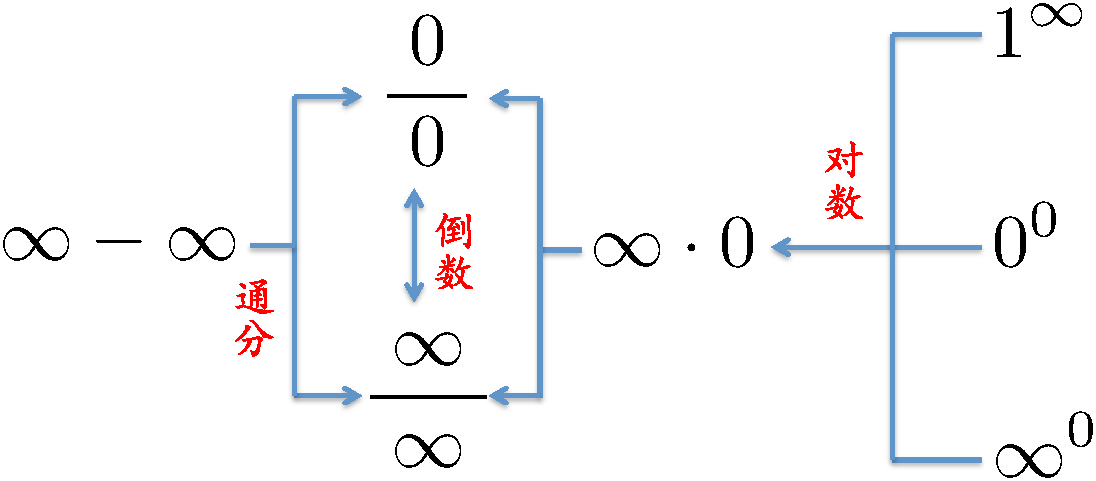
\includegraphics{./images/ch5/lim00.pdf}}
	\end{center}
\end{frame}

\begin{frame}
	\linespread{1.2}
	\begin{exampleblock}{{\bf 例11}\hfill 习题5.2-15}
		设$f(x)$在$x_0$附近存在二阶连续导函数,则
		$$\lim\limits_{h\to 0}\df{f(x_0+h)+f(x_0-h)-2f(x_0)}{h^2}=f\,''(x_0).$$
		若条件减弱为“$f(x)$在$x=x_0$处二阶可导”,结论是否仍然成立?
	\end{exampleblock}
\end{frame}

\begin{frame}[<+->]{小结}
	\linespread{1.5}
%  	{\ba{问题:}}{\b 如何求闭区间上函数的最值和最值点?}\bigskip\pause
	\begin{enumerate}
	  \item {\bf 中值定理}
	  \begin{itemize}
	    \item Rolle定理
	    \item Lagrange中值定理
	    $$f(b)-f(a)=f\,'(\xi)(b-a),\quad \xi\in(a,b)$$
	    \item Cauchy中值定理
	  \end{itemize}
	  \item {\bf L'Hospital法则}
	  $$\limx{*}\df{f(x)}{g(x)}=\limx{*}\df{f\,'(x)}{g'(x)}$$
	\end{enumerate}
% 	\bigskip
% 	\pause
% 	\centerline{\ba{请自行阅读第六章\S 6.3节}}
\end{frame}

\begin{frame}{补充例题}
	\linespread{1.2}
	\begin{exampleblock}{{\bf 例12}(Darboux定理)\hfill}
		设$f(x)$在$[a,b]$上可导,且$f\,'_+(a)f\,'_-(b)<0$,则存在$\xi\in(a,b)$,
		使得$f\,'(\xi)=0$。
	\end{exampleblock}
	\pause
	\bigskip
	\begin{exampleblock}{{\bf 例12'}\hfill}
		设$f(x)$在$[a,b]$上满足Rolle定理条件,且$f\,'_+(a)f\,'_-(b)>0$,
		则$f\,'(0)=0$在$(a,b)$内至少有两个根。
	\end{exampleblock}
\end{frame}

\begin{frame}
	\linespread{1.2}
	\begin{exampleblock}{{\bf 例13}\hfill}
		设$\df{a_0}{n+1}+\df{a_1}{n}+\ldots+a_n=0$,证明:方程
		$$a_0x^n+a_1x^{n-1}+\ldots+a_n=0$$
		在区间$(0,1)$内至少有一个根。
	\end{exampleblock}
\end{frame}

\begin{frame}
	\linespread{1.2}
	\begin{exampleblock}{{\bf 例14}\hfill}
		设$f(x)$在$U(x_0)$内连续,在$U^0(x_0)$内可导,且$\limx{x_0}f\,'(x)=l$,则
		$$f\,'(x_0)=l.$$
	\end{exampleblock}
\end{frame}

\begin{frame}
	\linespread{1.2}
	\begin{exampleblock}{{\bf 例15}\hfill}
		设$f(x)$在$[a,b]$连续,在$(a,b)$可导,且$a\geq 0$,则存在
		$x_1,x_2,x_3\in(a,b)$,使得
		$$f\,'(x_1)=(b+a)\df{f\,'(x_2)}{2x_2}=(a^2+ab+b^2)\df{f\,'(x^3)}{3x_3^2}$$
	\end{exampleblock}
	\pause
	\begin{exampleblock}{{\bf 例16}\hfill}
		设$f(x)$在$[a,b]$连续,在$(a,b)$可导,且$f\,'(x)\ne 0$,证明:
		存在$\xi,\eta\in(a,b)$,使得
		$$\df{f\,'(\xi)}{f\,(\eta)}=\df{e^b-e^a}{b-a}e^{-\eta}$$
	\end{exampleblock}
\end{frame}

% \begin{frame}
% 	\linespread{1.2}
% 	\begin{exampleblock}{{\bf 例16}\hfill}
% 		设$f(x)$在$[a,b]$连续,在$(a,b)$可导,且$f\,'(x)\ne 0$,证明:
% 		存在$\xi,\eta\in(a,b)$,使得
% 		$$\df{f\,'(\xi)}{f\,(\eta)}=\df{e^b-e^a}{b-a}e^{-\eta}$$
% 	\end{exampleblock}
% \end{frame}

\begin{frame}
	\linespread{1.2}
	\begin{exampleblock}{{\bf 例17}}
		设$f(0)=1$,且
		$$\limx{0}\df{\ln(1-x)+f(x)\sin x}{e^{x^2}-1}=0,$$
		证明:$f(x)$在$x=0$处可导,求$f\,'(0)$。
	\end{exampleblock}
\end{frame}

%=======================================

% \begin{frame}{title}
% 	\linespread{1.2}
% 	\begin{block}{{\bf title}\hfill}
% 		123
% 	\end{block}
% \end{frame}

